This dissertation concerns the problem of representing coupled advection and diffusion in a manner that is physics-based, modular, reconfigurable, and leads to numerically efficient and robust models.  In complex physical systems, advection and diffusion are coupled to varying degrees in multiple domains.  This occurs to the extent that there is both \begin{inparaenum}[(1)] \item translation of material with respect to a reference frame or exchange of material between phases or chemical forms and \item a gradient or species-to-species variation in an intensive property (e.g., temperature, density, or velocity) that tends to become uniform due to thermal activity\end{inparaenum}.  It is known that the declarative or equation-based modeling approach can provide computational advantages and is compatible with physics-based, object-oriented representations.  However, there is no generally accepted method of representing coupled advection and diffusion in a declarative modeling framework.

In this dissertation, we will present an approach to this problem and apply it to fuel cells.  Fuel cells exhibit many processes which involve advection and diffusion to varying degrees, including chemical reactions, phase change, electrical conduction, fluid transport, multicomponent diffusion, and heat transfer.  In addition to being a pertinent demonstration platform, fuel cells are interesting in their own right as an efficient and effective energy conversion technology.

In this chapter, we will further introduce the context and motivation for the research (\autoref{sec:Motivation}) and present the research questions (\autoref{sec:Questions}).  Then we will describe the fuel cell application (\autoref{sec:FCMotivation}), which has its own context, motivation, and research questions.  Finally, we will provide an overview of the modeling approach (\autoref{sec:ModelingApproach}) and an outline of the dissertation (\autoref{sec:Outline}).



\section{Context and Motivation}
\label{sec:Motivation}

Mathematical modeling of physical systems is becoming more important due to the increasing complexity of engineered systems, the emphasis on system design, and improvements in modeling languages, tools, and algorithms.  Models are used in hardware and control design to run tests more quickly and cheaply than physical experiment.  They are used in research to explore hypotheses of physical behavior and to provide virtual sensors where physical sensors have lower fidelity, more uncertainty, or are simply not available or practical.  Models can also be simulated in real time for model-based control and model-in-the-loop testing.

There are many types of mathematical models of physical systems and many methods of classification:
\begin{itemize*}
  \item By physical domain: electrical, magnetic, mechanical (rotational or translational), thermal, fluid, chemical, etc.
  \item By mathematical formalism: algebraic equations, \np{ODE}, \np{DAE} or \np{PDE}
  \item By mathematical complexity: linear or nonlinear
  \item By mathematical causality: causal or acausal
  \item By the inclusion of time: static or dynamic
  \item By spatial dimensionality: \nfirst{0D}, \nfirst{1D}, or multi-dimensional
  \item By the representation of time: discrete, continuous, or hybrid
  \item By the representation of space: discrete, continuous, or hybrid
  \item By the level of physical abstraction: physics-based or empirical
  \item By encapsulation: flat or modular
  \item By the representation of physical hierarchy: flat or hierarchical
  \item By the programming or modeling language: C, Java, MATLAB, Modelica, etc.
\end{itemize*}
The choice of the type of model to use for an application depends on many factors including features of the physical system, what needs to be determined by the model and with what accuracy, how much the model will be reused, the cost of modeling and simulation software, the available computational resources, and the existing models and literature.

Due to the increasing complexity of engineered systems and the emphasis on system design, it is helpful if a model is modular, hierarchical, and acausal like a real system.  Modularity allows a modeler or designer to more easily reconfigure a model to consider multiple physical architectures.  Hierarchy allows detail to be hidden or encapsulated, without loss, as a system becomes more complex.  With modular, hierarchical, and acausal features, a model can convey not only the equations that govern behavior but also the structure of the system in a way that is useful for both human understanding and computer interpretation for simulation and other processing.

\emph{\N{acausal}} models and modeling languages are also called \emph{\n{declarative}}, equation-based, or physical-interaction~\cite{Matei2012}.  Declarative language preserves the simultaneous mathematical nature of equations.  By definition, an equation declares a relation between two expressions without implying mathematical causality (i.e., assigning independent and dependent variables).  The \emph{\n{causal}} approach is also called \emph{\n{imperative}}, sequential modular~\cite{Westerberg1994}, or signal-flow~\cite{Matei2012}.  It relies on assignment operations which are organized to form algorithms with predetermined input\slash{}output assignments.  The advantages of declarative language are described in detail below.


\subsection{Advantages of Declarative Modeling}
\label{sec:DeclarativeAdvantages}

Declarative language has four main advantages over causal or imperative language in modeling physical systems.  Declarative models are true to the acausal nature of physics, and compared to imperative models, they are more intuitive, more flexible and reusable, and less prone to user error.  These advantages are presented in more detail in the following paragraphs.

The first advantage is that declarative language best represents the nature of physical behavior and preserves the meaning of physical laws~\cite{Zenith2006, Willems2007, Cellier1996, Kofranek2008}.  For example, although current leads voltage in an electrical capacitor, the current does not cause the voltage to change any more than the change in voltage causes a current.  Placing the causality assignment in the capacitor's physical description is to suffer from the ``post hoc ergo propter hoc (it happened before, hence it caused) fallacy''~\cite{Willems2007}.  Declarative language allows the relationship to be expressed directly, without causality.  Imperative models should be reserved for flows of information in control engineering, signal processing, and similar fields of study.  As stated by Matei and Bock, ``Physical conservation laws do not apply in these applications because the same information can flow (be copied) to multiple components, while physical things cannot.''~\cite{Matei2012}

The second advantage is that declarative models are more intuitive than imperative ones.  This is demonstrated by \autoref{fig:Circuit}, which shows declarative and imperative models of the same electrical circuit.  The connections of the declarative model (\autoref{fig:DeclarativeCircuit}) represent wires which imply Kirchhoff's voltage and current laws (KVL and KCL)\glsunset{KVL}\glsunset{KCL}.  The diagram shows how the components would be actually assembled.  In contrast, the connections of the imperative model (\autoref{fig:ImperativeCircuit}) represent signals.  The type of signal (voltage or current) depends on the connection's context within the circuit, since the block for each electrical component receives voltage and transmits current or vice versa.  The topological equations (\n{KVL} and \n{KCL}) are represented by difference and summation blocks, and this distracts attention from the blocks which represent the constitutive equations of the capacitor, inductor, and resistors.

The third advantage is that declarative models are more flexible and reusable because they preserve the information necessary to perform symbolic manipulation.  Powerful modeling tools exist (see \autoref{sec:EOOLanguages}) that can solve a model for the imposed causality, linearize a model, partition a dynamic model into the most numerically efficient systems of algebraic equations (i.e., resolve algebraic loops through tearing), and perform index reduction (i.e., eliminate structural singularities)~\cite{Cellier2006, Mattsson1993b}. %, Elmqvist1994?
In addition, methods are being developed for analytical \n{MOR}~\cite{Donida2010}.  Returning to the electrical example, the declarative model of \autoref{fig:DeclarativeCircuit} independently maintains information about the circuit (capacitor, inductor, resistors, and their connections) and the causality imposed on it by the boundary condition (voltage source).  If the boundary condition is changed (e.g., current source instead of voltage source), a modeling and simulation tool can automatically change the causality as needed.  However, the imperative model of \autoref{fig:ImperativeCircuit} must be manually re-solved and reconfigured as shown in \autoref{fig:ImperativeCircuitInverse}.  The correlation is not obvious, which hinders model development and use.  It is not practical, especially for complex systems, to maintain multiple versions of a model for the sake of causality.  Automatic linearization is helpful in evaluating dynamic characteristics and in control techniques such as \n{MPC}.  Algebraic loops tend to occur in the representations of complex physical systems; therefore, it helps if declarative modeling tools can handle them in a robust manner.  Index reduction can be used as a tool to scale the amount of detail included in a model without adding simulation overhead.


\begin{figure}[htbp]
  \subfloat[Declarative]{
    \includegraphics[width=0.6\linewidth]{1-Declarative-viD}%
    \label{fig:DeclarativeCircuit}%
  }\\
  \subfloat[Imperative]{
    \includegraphics[width=0.8\linewidth]{1-Imperative-viD}%
    \label{fig:ImperativeCircuit}%
  }%
  \caption[Imperative and declarative models of an electrical circuit]{Imperative and declarative and imperative models of an electrical circuit~\cite{ModelicaTutorial1.4}}%
  \label{fig:Circuit}%
\end{figure}

\begin{figure}[htbp]
  \includegraphics[width=0.8\linewidth]{1-Imperative-ivD}%
  \caption{Inverse imperative model of the circuit in \autoref{fig:Circuit}}%
  \label{fig:ImperativeCircuitInverse}%
\end{figure}

The fourth and final advantage of declarative models is that they are less prone to user error.  Some modeling mistakes may be avoided because the conservation laws are inherently and rigorously included.  If the developer of a model library uses the correct conservation equations in the lowest-level models, any circuit a user builds from the library is guaranteed to also include the correct conservation equations via Kirchhoff's current law, which is applied at every node.  In an imperative model, the conservation equations must be manually included at every level of the model; therefore, it is easier to violate conservation equations~\cite{Matei2012}.  In addition, a user may be tempted to cascade two instances of imperative models such as the ones in Figures~\ref{fig:ImperativeCircuit} and \ref{fig:ImperativeCircuitInverse}.  This is incorrect because the impedance of the second circuit affects the output of the first.  Two instances of the declarative model (\autoref{fig:DeclarativeCircuit}) can be easily and correctly cascaded by connecting the two in parallel (after removing the voltage source of the second instance).


\subsection{Current Limitations}
\label{sec:DeclarativeLimitations}

\N{EOO} or declarative, circuit-based modeling has been gradually extended from Kirchhoff's electrical circuit laws of 1845 to the magnetic, rotational, translational, thermal, fluid, and chemical domains.  In each domain, the \emph{\np{effort}} and \emph{\np{flow}}\glsadd{flow-adj}, or physical quantities analogous to voltage and current, are now well-established.  However, the fluid and chemical domains are more complicated because the material flow carries not only atoms or molecules but also significant amounts of other conserved quantities such as momentum and energy~\cite{Cellier2009}.  This process is called \emph{\n{advection}} and is depicted in \autoref{fig:Advection}.  By nature, the amount of these quantities depends on the source of the material.  Methods have been developed to use the property of the source by switching according to the direction of material flow (see \autoref{sec:Upstream}).

However, the switching approach has two drawbacks.  The first is that it generally requires reinitialization upon flow reversal.  This can usually be handled without a problem, but it requires additional computation.  In some cases there is chattering, or frequently repeated flow reversal, which can slow a simulation considerably.  The second drawback is that the intensive property is ill-defined when the material flow rate is zero.  This can be addressed by building a method of regularization into the switching algorithm.  This is of little immediate consequence because there is no advection at zero material flow rate.  However, it is at zero material flow rate that \emph{\n{diffusion}}, or transfer due to thermal activity with no net material flow, dominates.  Diffusion occurs towards lower values of the intensive property as depicted in \autoref{fig:Diffusion}.  Diffusion is not captured by the switching approach.

\begin{figure}[htbp]
  \subfloat[Advection]{
    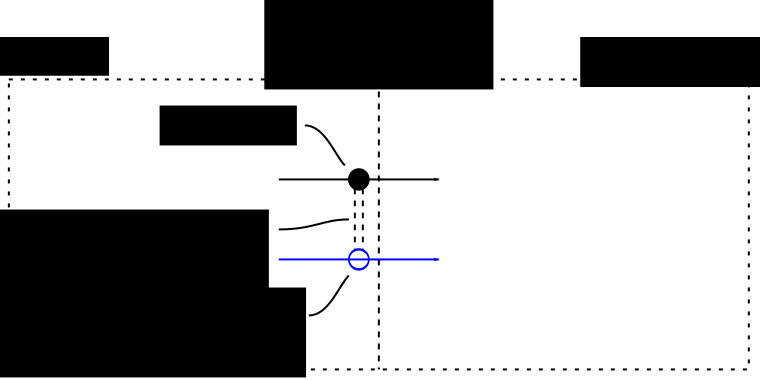
\includegraphics[width=0.48\linewidth]{1-Advection}%
    \label{fig:Advection}%
  }\quad
  \subfloat[Diffusion]{
    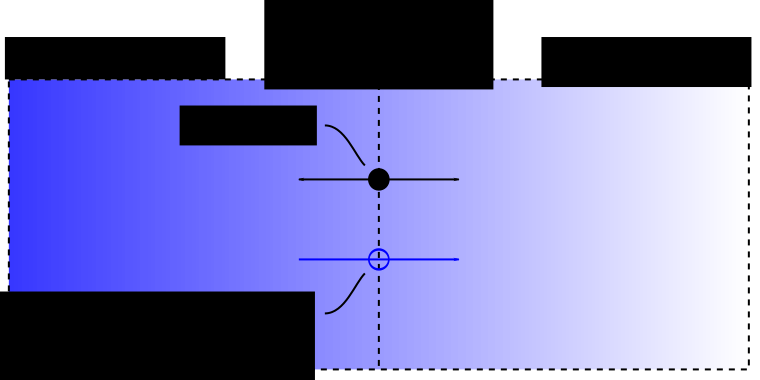
\includegraphics[width=0.48\linewidth]{1-Diffusion}%
    \label{fig:Diffusion}%
  }%
  \caption[Depiction of advection and diffusion]{Depiction of the two fundamental modes of transfer}%
  \label{fig:AdvectionDiffusion}%
\end{figure}

In some physical situations, there is mixed advection and diffusion.  To describe these situations, it is possible to add an additional pathway for purely diffusive transfer.  However, this is redundant and inconsistent because it yields two intensive properties at the boundary---one for advection and one for diffusion.  It also does nothing to eliminate the switching behavior or to resolve the advected property which is ill-defined at zero material flow rate.  This is the problem that the present research addresses---to model coupled advection and diffusion in a manner that is declarative, object-oriented, mathematically well-defined, numerically efficient, and physically representative yet generic.



\section{Research Questions}
\label{sec:Questions}

The goal of this research is to realize the advantages of declarative modeling for complex physical systems that involve both advection and diffusion to varying degrees in multiple domains.  We seek to answer the following questions:
\begin{enumerate}[\bfseries RQ1:]
  \item How can we create a generic declarative framework to model systems with processes that exhibit coupled advection and diffusion?
  \item How can the equations be best implemented to reflect the physical structure of a device and support reconfiguration?
  \item How appropriate is the framework for modeling all the relevant physical phenomena of an electrochemical device such as a fuel cell?
\end{enumerate}
The last question will be elaborated in the following section.



\section{Application to Fuel Cells}

In this dissertation, the modeling framework will be applied to fuel cells.  This will provide a pertinent and nontrivial demonstration of the framework while also establishing a novel approach to fuel cell modeling.  Declarative fuel cell models are physically appropriate~\cite{Zenith2006}, yet few models of this type exist (as shown in \autoref{chap:Background}).


\subsection{Context and Motivation}
\label{sec:FCMotivation}

\Np{FC} have the potential to serve a key role in our electric power networks, transportation systems, and portable electronic devices.  In general \np{FC} can convert fuel energy to work more efficiently and quietly than \np{ICE}~\cite{Larminie2003}, %[p.~23]
and a \n{FC} system's energy-to-power ratio can be easily adapted, unlike batteries.  A \n{FC} system can be refueled quickly like an \n{ICE} system, or it can be designed to recharge like a battery by operating in electrolysis mode~\cite{Burke2003}.  Of the various \nname{FC} technologies, \np{PEMFC} are best suited to meet the packaging and power-cycling requirements of vehicles and portable devices.

\Np{PEMFC} have a solid polymer-based electrolyte and operate at low temperatures (typically below \SI{100}{\celsius}).  As shown in \autoref{fig:CellFlows}, a single-cell \n{PEMFC} has few main components: a \n{PEM}, two catalyst layers or electrodes, two \np{GDL}, and two flow plates (FPs)~\cite{Larminie2003}. %[pp.~14--15 \& 67]
However, most applications require a higher voltage than a single-cell \n{PEMFC} can provide; therefore, two or more cells are joined back-to-back to form a \n{PEMFC} stack like the one shown in \autoref{fig:Stack}.

\begin{figure}[htbp]
  \includegraphics[width=0.75\linewidth]{1-CellFlows}%
  \caption[Layers of a single-cell \n{PEMFC}]{\glsreset{e-}%
  \glsreset{H+}%
  \glsreset{H2}%
  \glsreset{O2}%
  \glsreset{H2O}%
  Layers of a single-cell \n{PEMFC} and the primary paths of \n{e-}, \n{H+}, \n{H2}, \n{O2}, and \n{H2O} during normal operation}%
  \glsreset{e-}%
  \glsreset{H+}%
  \glsreset{H2}%
  \glsreset{O2}%
  \glsreset{H2O}%
  \label{fig:CellFlows}
\end{figure}

\begin{figure}[hbtp]
  \includegraphics[width=0.4\linewidth]{1-Stack}%
  \caption[\n{PEMFC} used to power an unmanned aerial vehicle]{\SI{500}{W}, 32-cell, water-cooled \n{PEMFC} used to power an unmanned aerial vehicle~\cite{Bradley2008}%[pp.\ 135--136]
}%
  \label{fig:Stack}
\end{figure}

A \n{PEMFC} operates on the chemical energy released by the reaction of \n{H2} and \n{O2} to produce \n{H2O}:
\begin{subequations}
  \begin{align}
    2\timessep\big(\s{H2} &\rightarrow 2\timessep\s{e-} + 2\timessep\s{H+}\big)\tag{HOR}\label{eq:HOR}\\
    4\timessep\s{e-} + 4\timessep\s{H+} + \s{O2} &\rightarrow 2\timessep\s{H2O}\tag{ORR}\label{eq:ORR}\\[-1.5em]
    \cline{1-2}\noalign{\vskip -0.9em}
    2\timessep\s{H2} + \s{O2} &\rightarrow 2\timessep\s{H2O}\tag{Net}\label{eq:CellReaction}
  \end{align}
\end{subequations}
Its \n{PEM} (electrolyte) controls the reaction by selectively passing protons while acting as a barrier layer to hydrogen, oxygen, and \n{e-}, as shown in \autoref{fig:CellFlows}.  This forces the reaction to occur in two sub-reactions:  the \n{HOR} whereby hydrogen is consumed and electrons and \n{H+} are produced, and the \n{ORR} whereby oxygen, electrons, and protons are consumed and water is produced.  In order to complete the full reaction, the electrons must travel an external path.  The path is provided by an external load which can harness the energy of the net reaction.

\glsunset{e-}
\glsunset{H+}
However, the cell has internal losses that cause heat generation and limit the rate at which the electrons can do a given amount of external work.  Some of the energy goes into making the reactions occur fast enough (activation losses), friction between the charge carriers (\n{e-} and \n{H+}) and the conducting materials (Ohmic losses), and transporting the reactants to and products away from the catalyst layers (concentration losses).

In order to operate, a \n{PEMFC} must be supported by other components, which are collectively called the \n{BOP}.  The \n{PEMFC} stack and \n{BOP} are the basis of a complete \n{PEMFC} system like the one shown in \autoref{fig:Ballard}.  \autoref{fig:FCSystem} shows the configuration of two \n{PEMFC} systems---one relatively simple and the other relatively complex.  Even more complex \n{PEMFC} systems may include heat recovery~\cite{Faghri2005} and fuel reformation.
\begin{figure}[htbp]
  \includegraphics[width=0.5\linewidth]{1-Ballard}%
  \caption[\n{PEMFC} system used to power a bus]{\SI{100}{kW} \n{PEMFC} system used to power a bus.  From Georgetown University, ``Generation III Project,'' \url{http://fuelcellbus.georgetown.edu}, accessed Nov.\ 2011%
}
  \label{fig:Ballard}
\end{figure}

\begin{figure}[htbp]
  \subfloat[Simple]{
    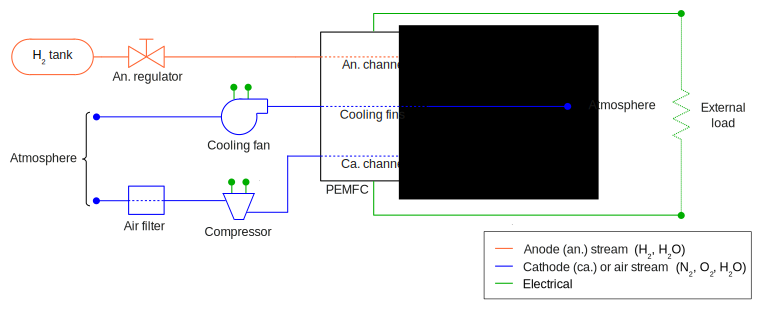
\includegraphics[width=0.75\linewidth]{1-SystemSimplest}%
    \label{fig:FCSystemSimplest}
  }\quad
  \subfloat[Complex]{
    \includegraphics[width=\linewidth]{1-SystemComplex}%
    \label{fig:FCSystemComplex}
  }
  \caption[Configurations of two \n{PEMFC} systems]{Configurations of two hydrogen-fueled (non-reforming), pressurized \n{PEMFC} systems where \subref{fig:FCSystemSimplest} the stack is air-cooled and \subref{fig:FCSystemComplex} the stack is water-cooled, the anode is preheated and recirculated, the anode and cathode are both humidified, and the cathode exhaust is expanded through a turbine}
  \label{fig:FCSystem}
\end{figure}
\glsadd{an.}
\glsadd{ca.}

Although \n{PEMFC} systems are promising, their cost and durability, and to a lesser extent, size and weight, must be improved to meet the desired standards for commercialization \cite[p.~11]{DOE2007}.  The U.S.\ Department of Energy has outlined the numerous avenues that are being pursued to improve the \n{PEMFC}, \n{BOP} components, and \n{PEMFC} system as a whole~\cite{DOE2007}.  The physical mechanisms of \n{PEMFC} degradation and failure are being determined and characterized through experimental and model-based investigations \cite[pp.~3, 9, 32, \& 40]{DOE2007}.  Novel materials and structures are being identified and developed for the core components of a \n{PEMFC} (\autoref{fig:CellFlows}) as well as the seals between and around them \cite[pp.~4--7]{DOE2007}.  These efforts seek to lower the cost of materials, improve thermodynamic efficiency (by decreasing the activation, Ohmic, and concentration losses), and improve robustness (specifically to air and fuel impurities, temperature and humidity variations, corrosive conditions, and power cycling).   Design techniques and manufacturing processes are being developed to support the low-cost and high-throughput production of \np{PEM}, electrodes, and flow plates \cite[pp.~2, 5--6, \& 29--30]{DOE2007},~\cite{Ding2010}.   One goal is to more effectively integrate the \n{PEM} and electrodes (as a \nname{MEA}\glsreset{MEA}) in order to minimize interfacial resistances, while at the same time allowing the raw materials to be reused or recycled \cite[pp.~3--10]{DOE2007}.

The \n{BOP} components are being improved as well.  New materials and  concepts are being applied to heat exchangers, humidifiers, compressors, and turbines with the goal of reducing their size, weight, and cost \cite[pp.~7, 10, \& 32]{DOE2007}.  Since the air compressor places a significant internal electrical load on the \n{PEMFC} system, it is important to maximize its efficiency, and in some cases, a turbine is beneficial \cite[p.~102]{Larminie2003}.  Air filtration technology is being evaluated to allow \np{PEMFC} to be used in off-road applications.  Sensors, especially those for chemical composition, are being further developed for reduced cost and size and improved accuracy, reliability, durability, and dynamic response. \cite[pp.~7]{DOE2007}.  The design of reformers and the operation of \n{PEMFC} on reformate is also being improved \cite[pp.~8--9]{DOE2007}, but in applications fueled by hydrocarbons rather than hydrogen, \np{PEMFC} are less likely to be prevalent over high-temperature \n{FC} technologies that can accept those fuels directly (and perform internal
reformation).

The final area of work considers how to improve the \n{PEMFC} system as a whole.  Alternative \n{PEMFC} system configurations and design parameters are being considered that may allow the functions of the \n{PEMFC} system to be performed by fewer or simpler components, or that may entirely eliminate the need for certain functions \cite[p.~10]{DOE2007}.  For example, one of eight or more possible methods for external humidification may be chosen, or the \n{PEMFC} can be operated within certain ranges of temperature and air flow rate where external humidification is not necessary \cite[pp.~83--90]{Larminie2003}.  Such choices must be guided by sufficiently accurate information, so \np{PEMFC} are being tested to evaluate their performance, durability, and other properties under various operating conditions, including hydrogen impurity \cite[p.~9]{DOE2007}.

Mathematical models are used to assist many of these efforts to develop \np{PEMFC}.  These models offer several benefits.  First, the operating conditions of a model can (in theory) be adjusted and measured easily.  As stated by Cellier, ``in the simulation world, all inputs and outputs are accessible''~\cite{Cellier1991}.  This can help provide insight into working mechanisms of a fuel cell~\cite{Faghri2005} via techniques such as model-based data analysis~\cite{Matzopoulos2007}.  Second, simulations are perfectly repeatable.  Models are not subject to unidentified disturbances and measurement error.  This means, for instance, that the effects of a design parameter can be clearly identified.  Third, fuel cell models are faster and cheaper to run than test equipment~\cite{Faghri2005, Matzopoulos2007}.  This is very important in design exploration, where many tests must be performed.  It also allows extreme operating conditions to be tested without risking damage to the fuel cell hardware.  Fourth, fuel cell models can help to organize and share knowledge about the configuration of a fuel cell and its working principles \cite{Matzopoulos2007}.  This is particularly important since fuel cells are multi-physical devices that require multi-disciplinary research and development.

However, due to the complexity of the structures and the physical processes that occur within \np{PEMFC}, specialized models are typically required for different situations.  Many academic articles have been published with \n{PEMFC} models that are appropriate and useful for particular cell designs, operating conditions, and levels of fidelity (i.e., spatial, dynamic, or behavioral detail~\cite{Pyster2012}) %[p. 83]
\cite{Faghri2005}.\footnote{The next chapter contains a literature review.}  Ideally, variants of a common \n{PEMFC} model could be used for a wide range of research and development work, including physical investigation, model-based systems design, and model-based control.  Such a model library could offer an open framework for \n{PEMFC} researchers to contribute their expertise and benefit from the collective knowledge of others.

A broadly applicable \n{PEMFC} model library would need to contain models that are \emph{physically representative}, meaning their predictions of behavior match reality (i.e., \emph{accurate}) and their structure corresponds to the physical domain.  Specifically and at a minimum, the static voltage-current predictions should be accurate over the following ranges of operating conditions:
\begin{itemize*}
\item \SIrange{0.3}{0.9}{V} electrical potential difference (per cell)\footnote{Low cell potentials (high electrical currents) are avoided in order to reduce the chemical\slash{}electrochemical transport losses.  High cell potentials are avoided because they accelerate the corrosion that occurs due to electrical cycling \cite[pp.~6--7]{Schmittinger2008}.}
\item \SIrange{20}{80}{\celsius} temperatures of flow plates and inlet gases (all varied together)\footnote{The lower bound corresponds to start-up from room temperature.  Nafion, the most common membrane material, dehydrates above \SI{\sim80}{\celsius}, which increases its protonic resistance~\cite{Hallinan2010}.}
\item \SIrange{1}{3.5}{atm} absolute anode\slash{}cathode outlet pressures (varied together)\footnote{Some \np{PEMFC} operate at atmospheric conditions.  \n{PEMFC} system efficiency is unlikely to increase above a pressure ratio of ${\sim}3.1$ \cite[p.~107]{Larminie2003}}
\item 0\% to 100\% relative humidity at anode inlet\footnote{For simplicity, some \n{PEMFC} systems do not have humidifiers (0\%).  Other systems humidify the anode as much as possible without causing flooding to occur (up to 100\%).}
\item 30\% to 70\% relative humidity at cathode inlet\footnote{The lower bound (30\%) corresponds to the relatively extreme case of operating the \n{PEMFC} without humidification in the Sahara desert on an average day \cite[p.~78]{Larminie2003}.  The cathode supply is usually not saturated; flooding would occur since \s{H2O}~is also produced in the cathode.}
\item 14\% to 100\% mean inlet\slash{}outlet oxygen concentration in dry cathode gas\footnote{The lower bound corresponds to a stoichiometric ratio of 1.5.  The risk of starvation increases as the ratio approaches 1.0.  \np{PEMFC} are also operated on pure oxygen in applications such as \np{UUV}.}
\end{itemize*}
The \n{PEMFC} model library should approximate the dynamic voltage-current response of actual cells at nominal operating conditions and varying large-signal electrical currents (e.g.,~\cite{Wagner1998}). %[p.~3787, Figures~2b and 2c]
It should capture the operational effects of design parameters including component sizes and material properties (for hardware analysis and design) and should be capable of linearization (for control analysis and design).  It should be able to describe relevant phenomena including electrochemical reactions, chemical\slash{}electrochemical transport, heat transport, and heat generation.  It should also have variable fidelity so that it can be used for layer-, cell-, stack-, system-, or application-level simulations.  Finally, it should be modular, meaning it should be possible to interconnect its submodels in various ways to build larger models analogous to the physical hierarchy.  Unfortunately, no current \n{PEMFC} model library can provide these features, let alone over the required range of operating conditions.


\subsection{Research Questions}%
\label{sec:FCQuestions}

As stated in research question three (RQ3), we will investigate how appropriate the declarative advective\slash{}diffusive framework is for modeling all the relevant physical phenomena of a fuel cell.  The hypothesis is that the framework can be used to help establish a fuel cell model library that is physics-based, modular, reconfigurable, accurate, and leads to numerically efficient and robust models.  As discussed in the previous section, such a library would be a valuable tool for fuel cell research and development.  In order to answer RQ3, we will address the following subquestions:
\begin{enumerate}[\bfseries RQ3a:]
  \item For which processes is it necessary to model mixed advection and diffusion?  Where is it appropriate to assume pure advection or pure diffusion?
  \item What characteristics do the models exhibit that would not be present given an imperative formalism?
  \item Which combinations of accuracy and speed can be achieved by adjusting fidelity?
\end{enumerate}



\section{Overview of the Modeling Approach}%
\label{sec:ModelingApproach}

As mentioned previously, the modeling approach is declarative, modular, and hierarchical.  This approach is also called \n{EOO} modeling.  The \autoref{fig:ModelHierarchy} illustrates that the models are created by building species (e.g., \s{H2}) into phases such as gas, phases into subregions, subregions into regions such as a fuel cell layer, and regions into assemblies such as a fuel cell.  This reflects the physical architecture of the device.
\begin{figure}[htbp]
  \newcommand{\I}[1]{\fbox{\includegraphics[height=2cm]{#1}}}
  \newcommand{\arrow}{\vbox to 1.95cm {\vfil
    \hbox{\LARGE $\rightarrow$}
    \vfil}}
  \I{4-SpeciesI}~\arrow~\I{4-PhaseI}~\arrow~\I{4-SubregionI}~\arrow~\fbox{\includegraphics[height=2.4cm]{4-RegionI}}~\arrow~\I{4-AssemblyI}%
  \caption{Levels of physical hierarchy in the model library}%
  \label{fig:ModelHierarchy}%
\end{figure}

The models are highly reconfigurable.  Assumptions may be applied that affect the spatial resolution and the included species, phenomena, axes of material translation, and boundaries.  With each assumption, the number and complexity of the equations scale appropriately and without simulation overhead.  The characteristics of individual species are provided in replaceable packages.  The packages can be used to model incompressible and compressible fluids including ideal and real gases.  The thermodynamic properties and other correlations are adjusted automatically according to these assumptions.

The models are dynamic and continuous in time.  Transients are modeled in terms of \np{DAE}, or implicit \np{ODE} combined with algebraic constraints.  These \np{DAE} are implemented in the Modelica language~\cite{Modelica3.3}.

The models are discrete in space.  As stated by Mattiussi~\cite{Mattiussi2000}, %[pp.~2--3]
this representation has three advantages: \begin{inparaenum}[(1)]\item it provides a unified perspective that is appropriate for many theories, \item it directly correlates the discretization of the physical region and the structural properties of the applied theories, and \item it is based on intuitive geometrical and physical concepts that help distinguish the numerical methods (e.g., \n{FDM}, \n{FVM}, and \n{FEM}) and the underlying theories\end{inparaenum}.  Rather than implementing approximations to traditional \n{PDE} representations, the approach is to distill the key concepts from equations such as Navier-Stokes and formulate them in a manner best uses features of \n{EOO} language.  The models have options for one, two, or three dimensions.  The grid of control volumes is rectilinear but the lengths are adjustable.

Computational efficiency is emphasized.  The translated models contain only linear systems of equations.  Techniques are used to reduce computational complexity, for example by representing high-order polynomials in nested form.  Many optional assumptions may be enabled to simplify the model.  For example, the temperature of different phases may be constrained to be the same; this results in index reduction and a simpler model.

The advective\slash{}diffusive framework is applied to the electrical, thermal, fluid, and chemical domains.  The approach is deeply physics-based.  It employs dynamic conservation equations for material, translational momentum, and energy.  Since the models are also resolved down to the species level, this requires traditional equations to be described at a more fundamental level.  For instance, Ohm's law and the Maxwell-Stefan equations for multi-component diffusion are not implemented directly.  Instead, drag interactions are modeled in a manner that results in those equations.



\section{Outline of the Dissertation}
\label{sec:Outline}

In this chapter, we have introduced the research by discussing the motivation, questions, and general approach.  The subjects of the remaining chapters are as follows:
\begin{itemize*}
  \item \textbf{\autoref{chap:Background} --- \nameref{chap:Background}:}  Survey of the relevant literature in the areas of declarative modeling languages, approaches to fluid flow in declarative language, and fuel cell models
  \item \textbf{\autoref{chap:Fundamentals} --- \nameref{chap:Fundamentals}:}  Detailed presentation and justification of the model equations which cover thermodynamics, material properties, transport, and exchange
  \item \textbf{\autoref{chap:Implementation} --- \nameref{chap:Implementation}:}  Summary of the implementation of the equations in a fuel cell model library
  \item \textbf{\autoref{chap:Basic} --- \nameref{chap:Basic}:}  Discussion of the conditions and results of several low-level demonstrations of the model library
  \item \textbf{\autoref{chap:Cell} --- \nameref{chap:Cell}:}  Discussion of the conditions and results of polarization tests and a dynamic example of the fuel cell model
  \item \textbf{\autoref{chap:Conclusions} --- \nameref{chap:Conclusions}:}  Recapitulation of the dissertation, list of contributions, and suggestions for future work
  \item \textbf{\autoref{chap:RelatedTheory} --- \nameref{chap:RelatedTheory}:}  Derivations and discussions that relate the model to selected theories in fluid dynamics and solid-state physics
  \item \textbf{\autoref{chap:Doc} --- \nameref{chap:Doc}:}  User documentation, diagrams, source code, and tables of parameters and connectors of the fuel cell model library
\end{itemize*}